\documentclass{article}

\usepackage[utf8]{inputenc}
\usepackage[french]{babel}
\usepackage[a4paper, left=2cm, right=2cm, top=2.5cm, bottom=2.5cm]{geometry}
\usepackage{amssymb}
\usepackage{amsmath}
\usepackage{graphicx} % pour les images 
\usepackage{listings} % pour intégrer un code R
\usepackage{xcolor} % pour coloriser le code R intégré
\usepackage{comment}
\usepackage{float}

\lstset{
	language=R,
	inputencoding=utf8, 
	extendedchars=true,       
	basicstyle=\ttfamily\footnotesize,
	keywordstyle=\color{blue},
	commentstyle=\color{green!50!black},
	stringstyle=\color{red},
	numbers=left,
	numberstyle=\tiny,
	stepnumber=1,
	breaklines=true,
	literate=%
	{é}{{\'e}}1
	{è}{{\`e}}1
	{ê}{{\^e}}1
	{à}{{\`a}}1
	{ù}{{\`u}}1
	{ç}{{\c{c}}}1
}

\title{Étude des valeurs extrêmes univariées}
\author{El Mazzouji Wahel, Mariac Damien, Condamy Fabian} 
\date{\today} 

\begin{document}

\maketitle 
\newpage
\tableofcontents 
\newpage
\section{Introduction}

Les événements extrêmes tels que les inondations, les crues, les canicules, les crises financières ou encore les krachs boursiers sont certes rares, mais peuvent avoir des conséquences considérables. Leur modélisation statistique constitue aujourd’hui un enjeu majeur dans des domaines aussi variés que la climatologie, l’assurance, la finance ou encore l’ingénierie.

Bien que de tels phénomènes ne puissent pas toujours être évités, la société peut mettre en œuvre des stratégies préventives afin d’en limiter les impacts. C’est dans cette optique que s’inscrit la théorie des valeurs extrêmes (TVE), un outil statistique essentiel dédié à l’analyse et à la prédiction des événements rares. Développée dès le début du XX\textsuperscript{e} siècle grâce aux travaux fondateurs de Fréchet (1927), Fisher et Tippett (1928), puis formalisée par Gnedenko (1943), cette théorie vise à modéliser les observations situées dans les queues des distributions de probabilité.

Dans la plupart des approches statistiques classiques, l’accent est mis sur le comportement global d’un échantillon, notamment par l’étude de ses moments (moyenne, variance, etc.). Ces méthodes reposent en grande partie sur le théorème central limite (TCL), énoncé par Pierre-Simon de Laplace en 1809, qui stipule que la somme (ou la moyenne) normalisée d’un grand nombre de variables aléatoires indépendantes et identiquement distribuées converge en loi vers une distribution normale.

Toutefois, le TCL ne donne aucune information sur le comportement des valeurs extrêmes, les plus grandes ou les plus petites observations qui sont pourtant cruciales dans les situations de risque. Il est donc naturel de se demander s’il existe un résultat asymptotique analogue au TCL pour les extrêmes d’un échantillon.

Pour cela, on considère un échantillon de variables aléatoires i.i.d. $(X_1, X_2, \dots, X_n)$, et l’on s’intéresse au comportement du maximum :
\[
M_n = \max\{X_1, X_2, \dots, X_n\}.
\]

La théorie des valeurs extrêmes cherche à étudier la convergence en loi de $M_n$ (après normalisation éventuelle), ainsi que les conditions sous lesquelles cette convergence a lieu. Elle permet d’identifier les lois limites possibles pour les maxima (ou minima), qui sont : la loi de \textit{Fréchet}, la loi de \textit{Gumbel} et la loi de \textit{Weibull}, chacune correspondant à un type de comportement de la queue de distribution.

\medskip
\noindent
\textbf{Remarque :} L’étude du minimum est entièrement analogue, il suffit d’examiner $-\min(X_1, \dots, X_n)$.

\medskip
\noindent
La théorie des valeurs extrêmes trouve des applications concrètes dans de nombreux domaines. Elle est utilisée en :
\begin{itemize}
    \item \textbf{Hydrologie}, pour prévoir les crues et protéger les zones inondables ;
    \item \textbf{Climatologie}, pour modéliser les épisodes météorologiques extrêmes ;
    \item \textbf{Assurance}, pour estimer la probabilité de sinistres rares et coûteux ;
    \item \textbf{Finance}, pour évaluer les risques extrêmes liés aux variations de marché ;
    \item \textbf{Ingénierie}, pour garantir la fiabilité des structures face à des sollicitations exceptionnelles.
\end{itemize}

En fournissant un cadre théorique rigoureux pour l’analyse des queues de distribution, la TVE permet d’anticiper la fréquence et l’intensité des événements rares, et ainsi d’aider à la prise de décision dans des contextes à fort enjeu.

\section{Les lois de $M_n$}

\subsection{Quelques notations }

On commence par faire une remarque sur la fonction de repartion de $M_n$ en utilisant le fait que les $X_i$ sont i.i.d :
\\
En effet, si on note $F_{M_n}$ la fonction de repartition de $M_n$, et $F_{X_i}$ la fonction de repartition de $X_i$ on a :
\[
\forall t \in \mathbb{R} \quad F_{M_n}(t) = \mathbb{P}(M_n < t) = \mathbb{P}(X_1 < t,...,X_n <t)=\mathbb{P}(X_1<t)^n = F_{X_1}^n(t) 
\]
\\
Dans la suite, on notera $F(t)$, la fonction de repartition des $X_i$.
\\
\\
Mais on rencontre un probleme ici, puisque si $n\to + \infty$, $F(t)^n$ converge vers 0 (ou 1 si t est la borne sup du support des $X_i$).
\\
\\
\\
L'idée est donc d'introduire 2 suites ($b_n$) et ($a_n$) (avec $a_n > $  0 pour tout n) afin de pouvoir contrôler $M_n$.

Puis étudier la loi de la limite de $\frac{M_n - b_n}{a_n}$. Comme la fonction de repartition caracterise la loi, il nous suffit d'étudier la fonction $G$ définie pour tout t dans le support des $X_i$ comme :

\[
\mathbb{P} \left( \frac{M_n - b_n}{a_n} < t \right) \xrightarrow[n\to +\infty]{} G(t)
\]
\\
Si il existe de tel suite $a_n$ et $b_n$ alors on dit que $F$ est dans le domaine d'attraction de $G$.
\\
\\
à ce stade la, il nous faut donc trouver les distributions G qui peuvent apparaître comme limite dans l’équation ci-dessus.
\\
\\
Pour ce faire, nous allons utiliser le théoreme suivant : 
\\
\\
\underline{\textbf{Théorème (méthode de la fonction muette)}:}
Soit \( Y_n \) une variable aléatoire de fonction de répartition \( F_n \), et soit \( Y \) une variable aléatoire de fonction de répartition \( F \).  
Alors $Y_n \xrightarrow{\mathcal{L} } Y$ si et seulement si pour toute fonction $z$ réelle, bornée et continue :
\[
\mathbb{E}[z(Y_n)] \to \mathbb{E}[z(Y)].
\]

En prenant ici $Y_n = \frac{M_n -b_n}{a_n}$, on obtient :
\[
\mathbb{E}[z(\frac{M_n -b_n}{a_n})] = \int_{-\infty}^{\infty} z(\frac{x-b_n}{a_n}) \: n \:  F^{n-1} (x)dF(x)
\]

L'astuce ici va être de faire un changement de variable astucieux. On va poser : 

\[
x = Q(1-\frac{1}{y}) = K(y) \; \; \; \; \; \; \text{avec Q la fonction quantile}
\]

\begin{equation}\label{eq:1.1}
    \text{Donc,} \; \; \int_{-\infty}^{\infty} z\Bigl(\frac{x-b_n}{a_n}\Bigr) \, n \, F^{n-1}(x)\,dF(x)
    =\int_{0}^{n} z\Bigl(\frac{K\Bigl(\frac{n}{v}\Bigr)-b_n}{a_n}\Bigr)
    \Bigl(1-\frac{v}{n}\Bigr)^{n-1}dv.
\end{equation}
\\
\\
Or, on a $\lim_{n \to \infty} ( 1 - \frac{v}{n})^{n-1} = e^{-v}$ , et on a $\lim_{n \to \infty} \int_{0}^{n} = \int_{0}^{+ \infty}$.

\subsection{Paramètre $b_n$}

On en déduit une bonne valeur pour $b_n$. En effet,
\[
\mathbb{P} \left( \frac{M_n - b_n}{a_n} < t \right) \xrightarrow[n\to +\infty]{} G(t) \in ]0:1[
\]
\[
\Longleftrightarrow F^n(a_n t + b_n) \xrightarrow[n\to +\infty]{} G(t)
\]
\[
\Longleftrightarrow n \: ln(F(a_n t + b_n)) \xrightarrow[n\to +\infty]{} ln(G(t))
\]
\[
\Longleftrightarrow n(- F(a_n t + b_n) + 1) \xrightarrow[n\to +\infty]{} ln(G(t)) \quad \quad (\text{car} \quad \lim_{x \to 0} \frac{ln(1-x)}{x} = -1)
\]
\[
\Longleftrightarrow n \: \mathbb{P}(X_1 > a_n t + b_n ) \xrightarrow[n\to +\infty]{} - ln(G(t))
\]
On obtient alors pour paramètre d'échelle :
\[
n \mathbb{P}(X_1 > b_n) =1  \Longleftrightarrow \mathbb{P}(X_1 < b_n) = 1 - \frac{1}{n}
\]
\[
\Longleftrightarrow F(b_n) = 1 - \frac{1}{n}
\]
\[
b_n = Q(1-\frac{1}{n}) = K(n)
\]
Dans la dernière équivalence, on a composé par la fonction quantile.
\\
\subsection{Paramètre $a_n$}
Avec le parametre $b_n$ définie au dessus et en posant $u=\frac{1}{v}$ on obtient alors une condition, il faut qu'il existe une fonction $a$ tel que $\lim_{x \to \infty} \frac{K(xu) - K(x)}{a(x)}$ converge \textbf{vers une fonction $h(u)$}.
\\
\\
\textbf{Proposition :}
\\
Les limites possibles sont données par :

\begin{equation}\label{eq:1.2}
    c\,h_{\gamma}(u) 
    \;=\; 
    c \int_{1}^{u} v^{-\gamma - 1}\,dv 
    \;=\; 
    c\,\frac{u^{\gamma} - 1}{\gamma}.
\end{equation}

Nous interprétons $h_{0}(u) = \log(u)$ lorsque $\gamma = 0$.
\\
\\
\textbf{Remarque :} On ne veut pas que $c=0$, car il conduit à une limite dégénérée pour $\frac{M_{n} - b_n}{a_n}$. 
Ensuite, le cas $c>0$ peut être ramené au cas $c=1$ en incorporant $c$ dans la fonction $a$.   
\\
\\
\textbf{Preuve de la Proposition}  
\\
Soient $u,v >0$. Alors :
\[
\frac{K(xuv) - K(x)}{a(x)} 
\;=\; 
\frac{K(xuv) - K(xu)}{a(xu)} \,\frac{a(xu)}{a(x)}
\;+\;
\frac{K(xu) - K(x)}{a(x)}.
\tag{2.3}
\]
Si la limite dans $F$ est dans le domaine d'attraction de $G$ (\textit{ce qu'on suppose depuis le début}), alors le rapport $\frac{a(ux)}{a(x)}$ converge vers $g(u)$.
\\
\\
De plus,
\[
\frac{a(xuv)}{a(x)} 
\;=\;
\frac{a(xuv)}{a(xv)} \,\frac{a(xv)}{a(x)}.
\]
Par passage à la limite pour $x$, la fonction $g$ satisfait l'\textit{équation fonctionnelle de Cauchy} :
\[
g(uv) = g(u)\,g(v).
\]
\\
Les solutions de cette équation sont de la forme $g(u)= u^{\gamma}$ avec $\gamma$ un réel.
\\
Donc, on a $\lim_{x\to \infty} \frac{a(ux)}{a(x)} \;=\; x^{\gamma} l(x)$, on dit dans ce cas que $a$ est une fonction à variation régulière.
\\
\\
En réécrivant l'expression (2.3) avec cette convergence, on en déduit que la fonction limite est de la forme
\[
h_\gamma(u)= c\,\frac{u^\gamma-1}{\gamma},
\]
avec la convention \(h_0(u)=\ln u\).
\\
Ainsi, nous concluons que
\[
h_\gamma(u)=\frac{u^\gamma-1}{\gamma} \quad \text{(avec \(h_0(u)=\ln u\))},
\]
\hfill $\square$
\\
\subsection{Les lois limites}
En reprenant $(2.3)$ et en utilisant ce qui précède, on obtient :
\[
\lim_{x\to \infty} \frac{K(xuv) - K(x)}{a(x)} = u^{\gamma} h(v) + h(u)
\]
\[
\text{autrement dit :} \; \; h_{\gamma}(uv)= u^{\gamma} h_{\gamma}(v) + h_{\gamma}(u)
\]
\\
\\
On fait alors une disjonction de cas sur la valeur de gamma.
\\
\subsubsection{Nature du support}

En reprenant l'équation \eqref{eq:1.2}, on obtient :
\[
h_\gamma\Bigl(\frac{1}{v}\Bigr)=\frac{(1/v)^\gamma-1}{\gamma}=\frac{v^{-\gamma}-1}{\gamma}
\]
Posons \(u=\frac{v^{-\gamma}-1}{\gamma}\). On résout alors pour \(v\) :
\[
v^{-\gamma}=1+\gamma u\quad\Longrightarrow\quad v=(1+\gamma u)^{-1/\gamma}
\]
Le changement de variable de \(v\) à \(u\) permet de réécrire l'intégrale limite sous la forme
\[
\int_{u\in S_\gamma} z(u)\,d\Bigl\{\exp\Bigl[-\left(1+\gamma u\right)^{-1/\gamma}]\Bigr\}
\]
ce qui conduit à identifier la loi limite par
\[
G_\gamma(u)=\exp\Bigl\{-\left(1+\gamma u\right)^{-1/\gamma}\Bigr\}
\]
Il reste alors à étudier la nature du support \(S_\gamma\), mais celui-ci dépend du signe de \(\gamma\) :

\subsubsection{Si \(\gamma>0\)}
L'inversion montre que \(v\in [0,1]\) correspond à \(u>-\frac{1}{\gamma}\).
\\
\\
De plus, pour de grandes valeurs \(x\) on a :
\[
S(x) \approx \exp\Bigl[-\bigl(1 + \gamma x\bigr)^{-1/\gamma}\Bigr]
\]
Or, par un développement asymptotique,  \(\bigl(1 + \gamma x\bigr)^{-1/\gamma}\) est proportionnel à \(x^{-1/\gamma}\) pour \(x\) grand. On obtient alors
\[
S(x) \approx \exp\bigl[-C\,x^{-1/\gamma}\bigr] 
\quad (\text{pour une constante } C>0).
\]
Par croissance comparé, comme \(x^{-1/\gamma}\) tend vers 0 moins vite que \(\exp(-\alpha x)\). On a alors : 
\[
S(x)\,\sim\, K\,x^{-1/\gamma} 
\quad (\text{pour } x\to\infty),
\]
ce qui caractérise une \textbf{queue bornée} : la probabilité d'observer des valeurs très grandes est plus élevée que dans un modèle à décroissance exponentielle.

\subsubsection{Si \(\gamma<0\)}
Pour \(\gamma < 0\), la loi est définie quand :
\[
1 + \gamma u > 0 \quad \Longrightarrow \quad u < - \frac{1}{\gamma}
\]
Cela signifie que la distribution a son support dans \(]-\infty, - \frac{1}{\gamma} [ \) 
\\
On pose alors \(x_{\max} = - \frac{1}{\gamma} \).
\\
Par conséquent, la fonction de survie $S(x) = 1 - G(x)$ = 0 pour \(x \ge - \frac{1}{\gamma} \).
\\
\\
Autrement dit, il n'y a aucune probabilité d'observer une valeur au-delà de \(x_{\max}\). Dans ce cas, on dit que la distribution est à \textbf{queue bornée}.
\\
\\
On dit alors que que queue de distribution est bornée.
\subsubsection{2. Cas \(\gamma=0\)}
Lorsque \(\gamma = 0\), on a posé $h_0(u)=\ln u$.
\\
Donc, le changement de variable s'adapte : 
\[
u=h_0\Bigl(\frac{1}{v}\Bigr)=\ln\Bigl(\frac{1}{v}\Bigr)=-\ln v,
\]
ce qui implique
\[
v=e^{-u}.
\]
Le changement de variable transforme alors l'intégrale limite en
\[
\int_{-\infty}^{\infty} z(u)\,d\Bigl\{\exp\Bigl[-e^{-u}\Bigr]\Bigr\},
\]
et la loi limite est alors donnée par
\[
G_0(u)=\exp\Bigl\{-e^{-u}\Bigr\},\qquad u\in\mathbb{R},
\]
On retrouve ici une queue à décroissance exponentielle, ce qui est caractéristique d'une \textbf{queue légère} : la probabilité d'observer des valeurs extrêmes est faible.
\\
\subsection{Résumé}
Les lois limites qui s'imposent dependent d'un parametre $\gamma$ et sont les suivantes :
\\
\begin{itemize}
    \item \textbf{Si \(\gamma>0\)} (loi de Fréchet) :
    \[
    G_\gamma(u)=\exp\left\{-\left(1+\gamma u\right)^{-1/\gamma}\right\}, \quad u > -\frac{1}{\gamma}.
    \]
    
    \item \textbf{Si \(\gamma=0\)} (loi de Gumbel) :
    \[
    G_0(u)=\exp\left\{-e^{-u}\right\}, \quad u\in\mathbb{R}.
    \]
    
    \item \textbf{Si \(\gamma<0\)} (loi de Weibull) :
    \[
    G_\gamma(u)=\exp\left\{-\left(1+\gamma u\right)^{-1/\gamma}\right\}, \quad u < -\frac{1}{\gamma}.
    \]
\end{itemize}
\newpage
\section{Quelques exemples numériques}

\noindent Voici maintenant quelques applications numériques sur des lois usuelles de ce que nous avons vu dans cette section. Pour chacune des représentations suivantes, nous avons simulé 1000 fois chaque loi puis ensuite effectué 10000 simulations pour le maximum afin d'avoir une précision correcte. 

\subsubsection{Loi uniforme}

\noindent Pour la loi uniforme sur [0,1], on peut montrer théoriquement que la limite du max est une loi exponentielle de paramètre 1 (loi de Weibull bien particulière). \\
\noindent Soient \( U_1, U_2, \dots, U_n \) des variables aléatoires indépendantes et identiquement distribuées selon la loi uniforme sur \([0,1]\).

\noindent On a, pour $ x \in [0,1]$ :

\begin{align*}
	P(M_n \leq x) &= P(U_1 \leq x, \dots, U_n \leq x) \\
	&= P(U_1 \leq x)^n \text{ par indépendance des $U_i$}\\
	&= x^n
\end{align*}

\noindent Nous allons maintenant effectuer le changement de variable $ x = 1 - y/n $ avec $y > 0 $ pour examiner la queue de la distribution :

\[
P(M_n \leq 1 - y/n) = (1 - y/n)^n.
\]

\noindent Pour $ n $ grand, on a: $(1 - y/n)^n \approx e^{-y} $. Donc, $ P(M_n \leq 1 - y/n) \approx e^{-y} $.


\noindent Or, par définition, la loi exponentielle de paramètre 1 a pour fonction de répartition : $ P(Y \leq y) = 1 - e^{-y}, \quad y > 0. $

\noindent Ainsi, on a donc montré que :

\[
P(n(1 - M_n) \leq y) \to P(Y \leq y) = 1 - e^{-y},
\]

\noindent ce qui établit la convergence en loi :

\[
Y_n = n(1 - M_n) \xrightarrow{\mathcal{L}} \mathcal{E}(1).
\] 
\noindent Ainsi, on trouve que $a_n$ = $\frac{1}{n}$ et $b_n$ = 1.

\noindent Avec notre machine, nous obtenons le graphe suivant :

\begin{center}
	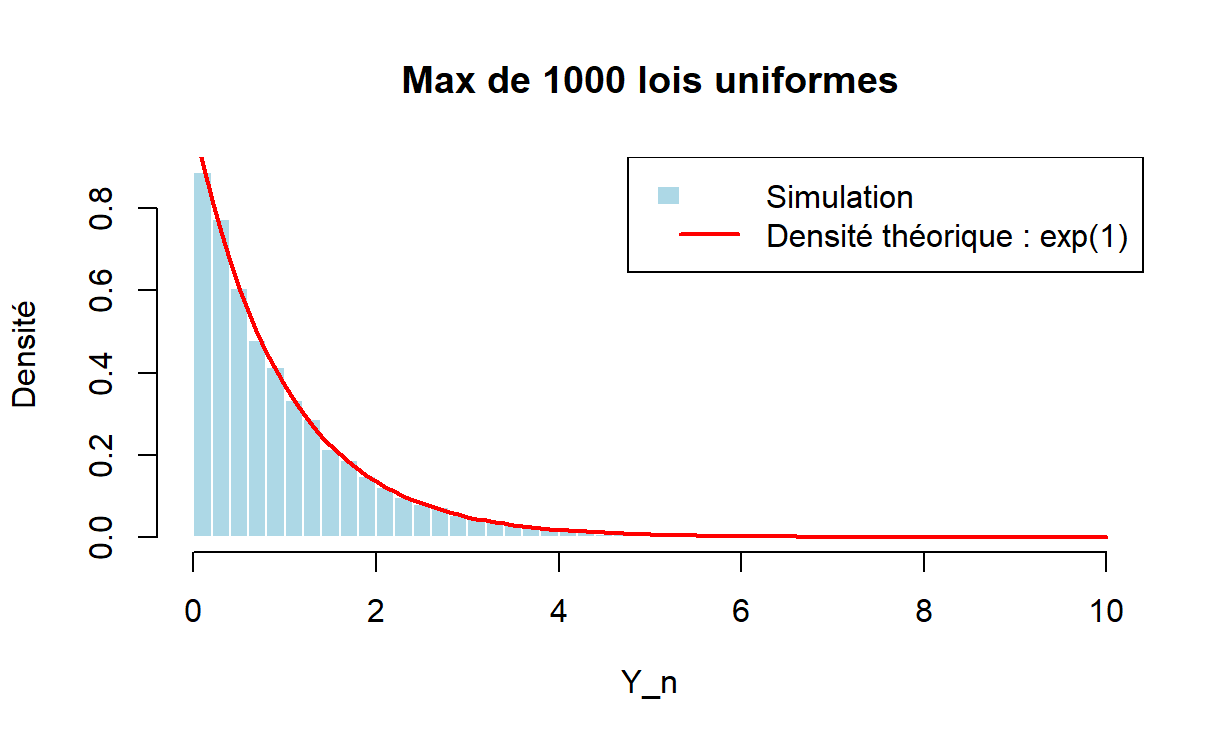
\includegraphics[scale=0.8]{./images/Max_Uniforme.png} 
\end{center}

\noindent Remarquons que l'on obtient une loi de Gumbell, ce qui est assez logique au vu du fait que ce soit une loi à queue très légère (elle n'en a tout simplement pas car son support est borné).

\subsubsection{Loi exponentielle}
\noindent Pour une loi exponentielle de paramètre 1, la loi limite est une loi de Gumbel. Théoriquement, on trouve $a_n = 1 $ et $b_n = \log(n) $.

\begin{center}
	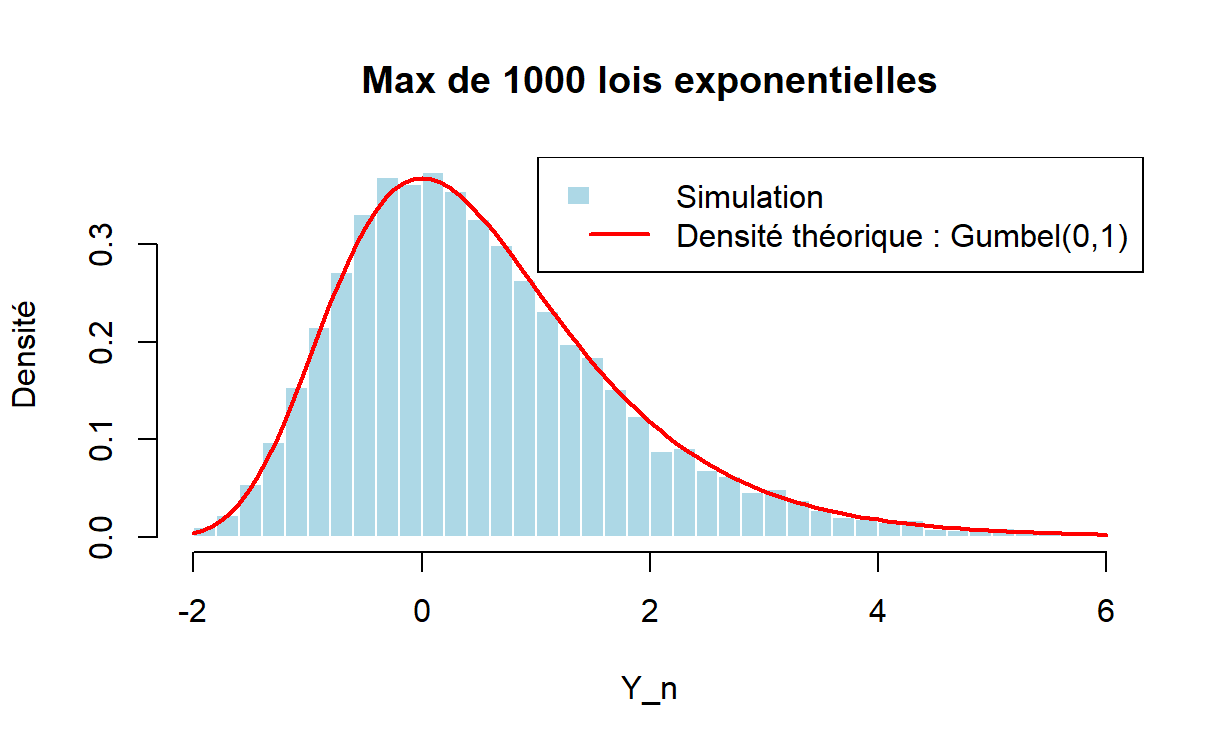
\includegraphics[scale=0.8]{./images/Max_Expo.png} 
\end{center}

\noindent Cette fois-ci, on avait une loi à queue fine, et on obtient loi de Gumbel, ce qui était attendu.

\subsubsection{Loi normale}

\noindent Pour maintenant une loi normale centrée-réduite, on peut montrer que la loi limite est encore une fois une loi de Gumbel. On trouve les paramètres généralisés $a_n = \frac{1}{\sqrt{(2*\log(n)}} $ et $b_n = \frac{1}{a_n} - \frac{\log(\log(n)) + \log(4 * pi)}{2 * \sqrt{2 * \log(n)}} $.

\begin{center}
	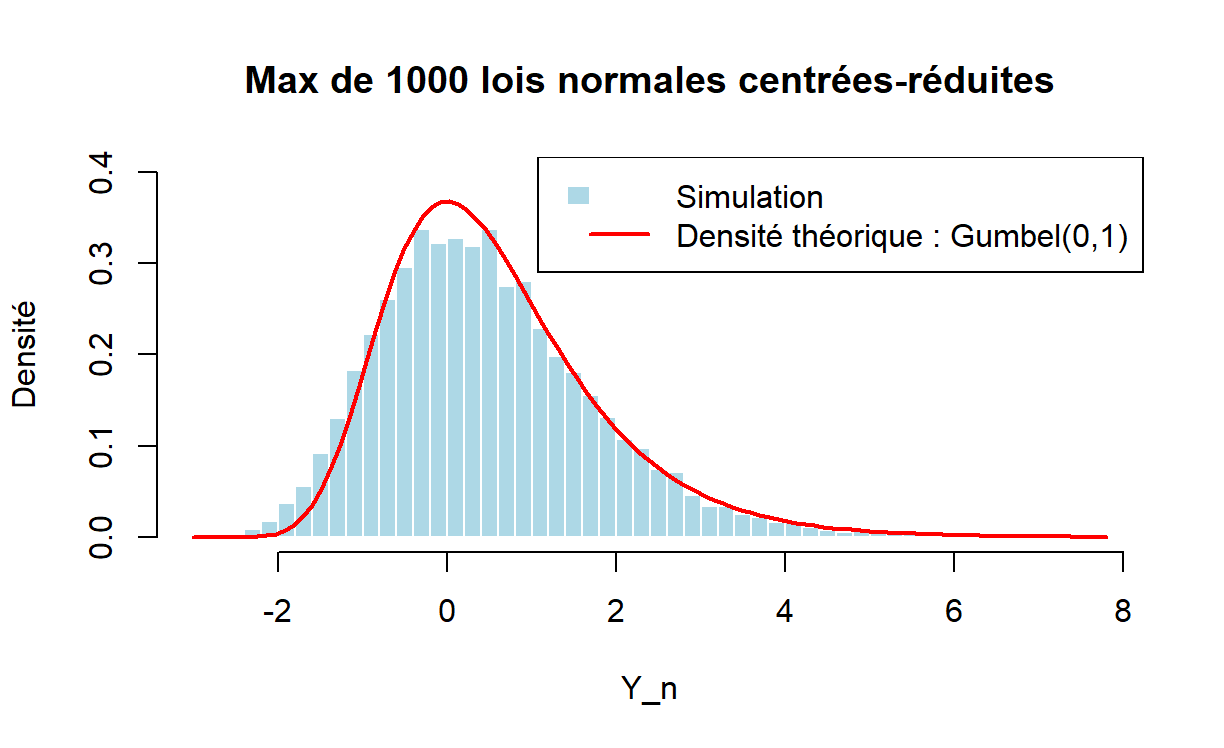
\includegraphics[scale=0.8]{./images/Max_Normale.png} 
\end{center}

\noindent Notons ainsi que l'on a la même loi limite que pour la loi exponentielle de paramètre 1, les graphes sont quasiment identiques.

\subsubsection{Loi de Cauchy}

\noindent Enfin, pour une loi de Cauchy (de paramètres 0 et 1 ici), la loi limite est une loi de Fréchet. On a les coefficients suivants : $a_n = pi $ et $b_n = n $.

\begin{center}
	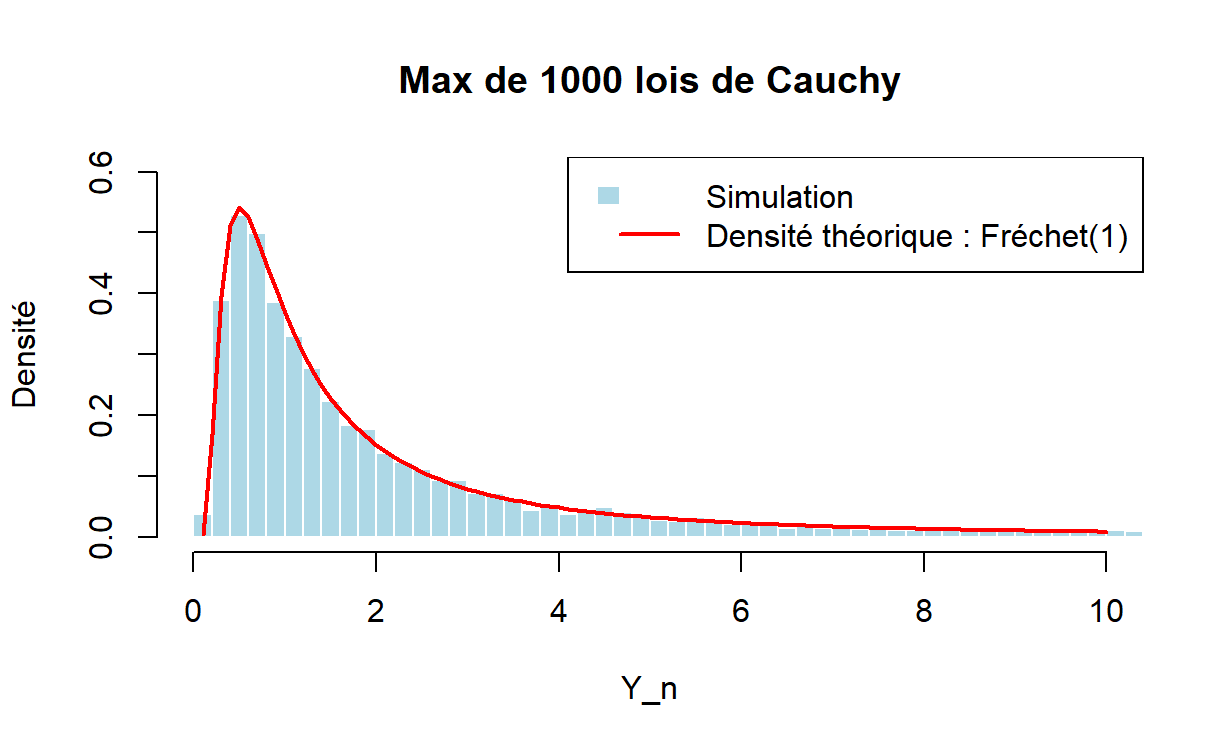
\includegraphics[scale=0.8]{./images/Max_Cauchy.png} 
\end{center}

\noindent Enfin ici, on avait une loi à queue lourde, et on obtient bien la loi de Fréchet attendue.

\newpage

\section{Méthodes d'estimation de l'indice de valeurs extrêmes}
Dans cette section, nous nous intéressons aux différentes méthodes d'estimation du paramètre \(\gamma\), intervenant dans la distribution des valeurs extrêmes généralisée. \\
D'une part, des approches non paramétriques sont dédiées à l'estimation de l'indice de queue, notamment les estimateurs de Hill et de Pickands. D'autre part, des méthodes paramétriques ont été développées, parmi lesquelles la méthode du maximum de vraisemblance, la méthode des moments et les approches bayésiennes. \\

\textbf{Définition :} On appelle \textit{statistique d'ordre} la permutation aléatoire de l'échantillon \(X_1, \dots, X_n\), qui ordonne les valeurs de l’échantillon par ordre croissant :

\[
X_{(1)} \leq X_{(2)} \leq \dots \leq X_{(n)}
\]

\textbf{Définition :} On dit qu'une suite \((k_n)_{n \geq 0}\) d'entiers est intermédiaire si :

\[
\lim_{n \to \infty} k_n = \infty \quad et \lim_{n \to \infty} \frac{k_n}{n} = 0
\]

\textbf{Définition :}
On dit qu'un estimateur \(\hat{\gamma_{n}}\) est convergent s'il converge en probabilité vers \(\gamma\), soit :
\[
\lim_{n \to \infty} P(\lvert \hat{\gamma_{n}} - \gamma \rvert > \epsilon) = 0 \quad \forall \epsilon > 0
\]

\subsection{Estimateur de Pickands}

L’estimateur de Pickands est construit à partir de trois statistiques d’ordre dans un échantillon. Il constitue l’un des premiers estimateurs non paramétriques proposés pour estimer l’indice des valeurs extrêmes \(\gamma\). Son principal avantage réside dans le fait qu’il est valide quel que soit le domaine d’attraction de la loi sous-jacente : Fréchet (\(\xi > 0\)), Gumbel (\(\xi = 0\)) ou Weibull (\(\xi < 0\)). Il n'est donc pas restreint à une famille particulière de distributions et reste applicable dans un cadre très général.

Néanmoins, cet estimateur est connu pour être assez sensible à la taille de l’échantillon, et en particulier au choix du paramètre intermédiaire \(k\), ce qui peut entraîner une certaine instabilité dans les estimations. Cela limite parfois sa robustesse, en particulier pour des tailles d’échantillon modestes.

En 1975, Pickands a démontré la consistance faible de son estimateur, c’est-à-dire la convergence en probabilité vers le vrai paramètre lorsque la taille de l’échantillon tend vers l’infini. Plus tard en 1989, Dekkers et de Haan ont établi la convergence forte ainsi que la normalité asymptotique de cet estimateur sous des conditions plus générales.

\medskip
\textbf{Définition.} Soit \(X_1, \dots, X_n\) une suite de variables aléatoires i.i.d. de loi \(F\), appartenant à l’un des domaines d’attraction des lois de valeurs extrêmes. On note \(X_{1,n} \leq \dots \leq X_{n,n}\) les statistiques d’ordre croissantes. Soit \((k_n)_{n \geq 1}\) une suite intermédiaire telle que \(k_n \to \infty\) et \(k_n / n \to 0\), l’estimateur de Pickands est défini par :

\[
\hat{\gamma}_{k,n} = \frac{1}{\ln(2)} \ln\left( \frac{X_{n-k+1,n} - X_{n-2k+1,n}}{X_{n-2k+1,n} - X_{n-4k+1,n}} \right)
\]

\medskip
L’estimateur de Pickands repose sur l’idée que, dans les queues d’une distribution extrême, les plus grandes observations suivent un comportement régulier. En considérant des statistiques d’ordre décroissantes, on peut approximer la structure de la queue à l’aide de différences successives entre grandes valeurs. L’utilisation d’une transformation logarithmique permet alors d’isoler l’indice de queue \(\gamma\), sous des conditions d’attraction à une loi limite.

\medskip
\textbf{Propriété de consistance.} Si \((k_n)\) est une suite intermédiaire, alors :
\[
\hat{\gamma}_{k,n} \xrightarrow{\mathbb{P}} \gamma
\quad \text{lorsque } n \to \infty.
\]

De plus, sous hypothèses régulières, l’estimateur est asymptotiquement normal :
\[
\sqrt{k} \left( \hat{\gamma}_{k,n} - \gamma \right) \xrightarrow{\mathcal{L}} \mathcal{N}(0, \sigma^2(\gamma))
\]
où la variance asymptotique est donnée par :
\[
\sigma(\gamma) = \frac{\gamma \sqrt{2^{2\gamma + 1} + 1}}{2(2^{\gamma} - 1)\ln(2)}.
\]

\medskip
Cette formule théorique permet de construire des intervalles de confiance pour l’estimation de \(\gamma\), bien qu’en pratique la variance soit souvent estimée par simulation.

\medskip
Enfin, une version généralisée de cet estimateur existe, introduisant deux paramètres \(u, v > 1\), permettant une plus grande flexibilité :
\[
\hat{\gamma}_{(k,u,v)} = \frac{1}{\ln(v)} \ln\left( \frac{X_{n-k+1,n} - X_{n-[uk]+1,n}}{X_{n-[vk]+1,n} - X_{n-[uvk]+1,n}} \right)
\]
Cette généralisation permet d'ajuster la stabilité de l'estimation. On retrouve l'estimateur de Pickands classique en prenant \(u = v = 2\).

\subsection{Représentation graphique de l’estimateur de Pickands}

Afin d'illustrer le comportement de l’estimateur de Pickands dans différents contextes, nous l'appliquons à des échantillons simulés de taille \(n = 40\,000\), issus de quatre lois représentatives : la loi de Pareto, la loi exponentielle, la loi uniforme sur \([0,1]\), et la loi de Cauchy. Ces lois permettent de couvrir les trois domaines d’attraction des lois de valeurs extrêmes, avec des indices théoriques respectifs de queue \(\gamma\) valant \(0.5\), \(0\), \(-1\), et \(1\).

Les figures ci-dessous présentent l’évolution de l’estimateur \(\hat{\gamma}_{k,n}\) en fonction de \(k\), c’est-à-dire du nombre d’observations extrêmes utilisées dans le calcul. Une ligne rouge horizontale indique la valeur théorique de \(\gamma\) pour chaque distribution, afin de visualiser la qualité de convergence.

\subsubsection{Loi de Pareto (\(\alpha = 2\))}

\begin{figure}[H]
    \centering
    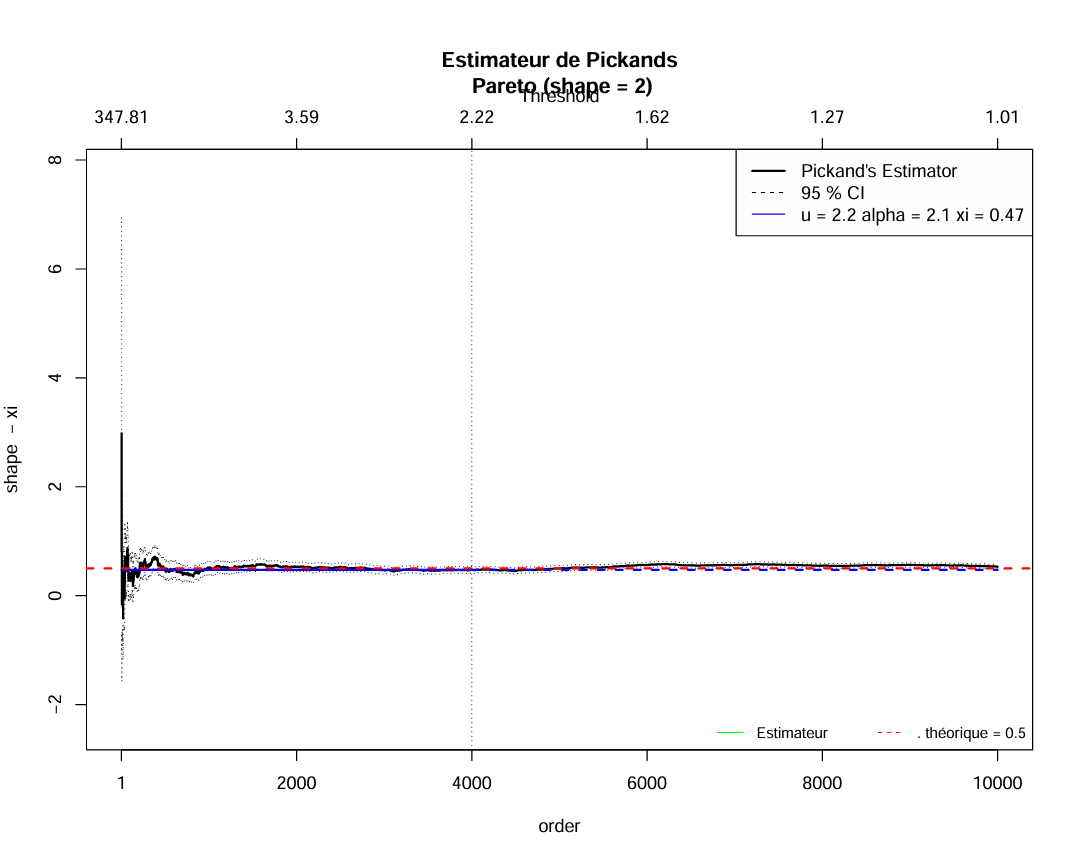
\includegraphics[width=0.8\textwidth]{./images/pareto.png}
    \caption{Estimateur de Pickands pour la distribution de Pareto (shape = 2).}
    \label{fig:pickands_pareto}
\end{figure}

La figure \ref{fig:pickands_pareto} illustre l’estimateur de Pickands appliqué à un échantillon simulé selon une loi de Pareto de paramètre \(\alpha = 2\), ce qui correspond à un indice de queue \(\gamma = 1/\alpha = 0.5\). L’estimateur converge clairement vers cette valeur lorsque \(k\) augmente, ce qui confirme la bonne performance de l’estimateur dans le cas d’une distribution à queue lourde.

\subsubsection{Loi exponentielle}

\begin{figure}[H]
    \centering
    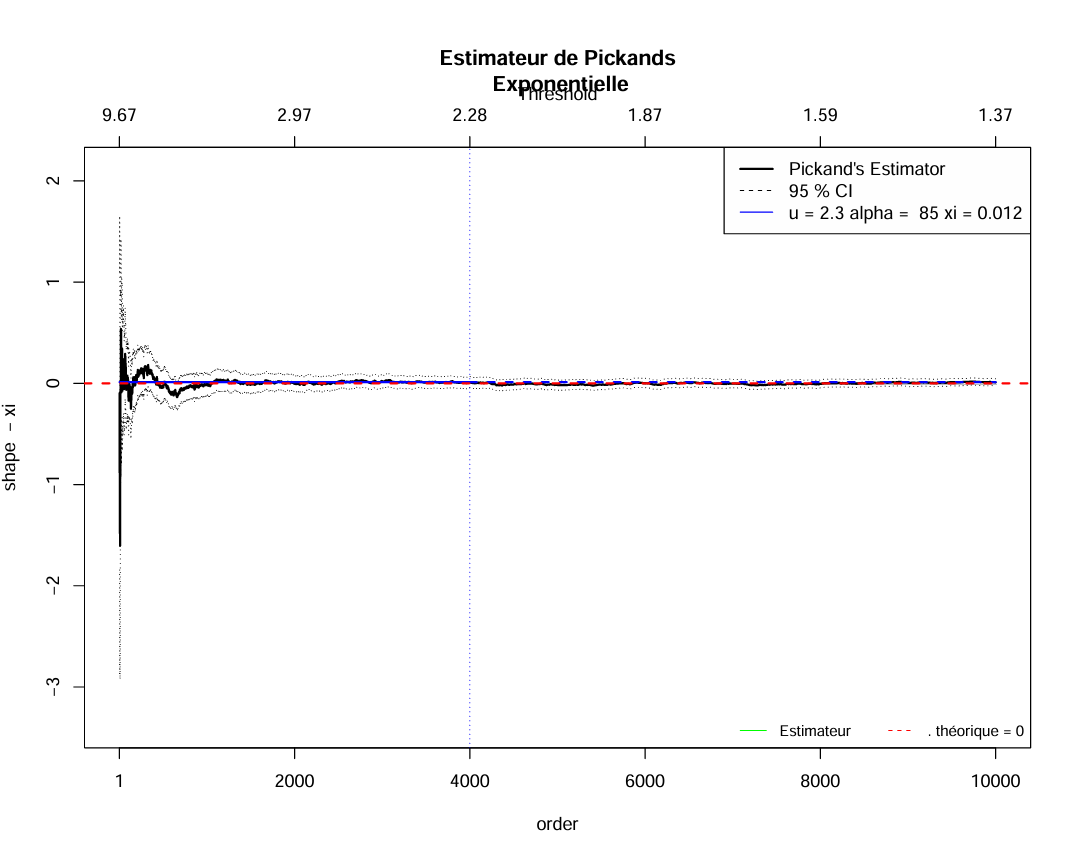
\includegraphics[width=0.8\textwidth]{./images/exponentielle.png}
    \caption{Estimateur de Pickands pour la distribution exponentielle.}
    \label{fig:pickands_exponentielle}
\end{figure}

Dans la figure \ref{fig:pickands_exponentielle}, on observe que l’estimateur de Pickands reste proche de zéro, en accord avec l’indice théorique \(\gamma = 0\) de la loi exponentielle. Ce résultat est cohérent avec le fait que cette loi appartient au domaine d’attraction de Gumbel.
\subsubsection{Loi uniforme \([0,1]\)}

\begin{figure}[H]
    \centering
    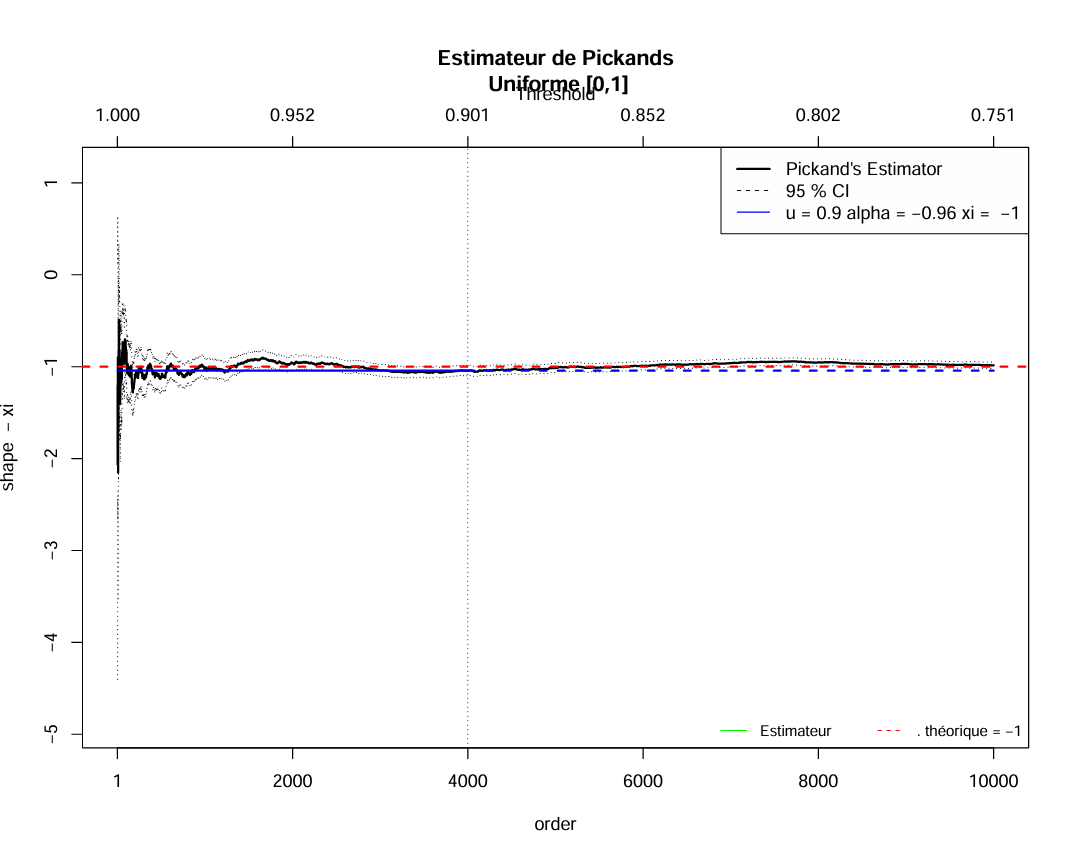
\includegraphics[width=0.8\textwidth]{./images/uniforme.png}
    \caption{Estimateur de Pickands pour la distribution uniforme sur \([0,1]\).}
    \label{fig:pickands_uniforme}
\end{figure}

Comme le montre la figure \ref{fig:pickands_uniforme}, l’estimateur décroît vers \(\gamma = -1\), valeur attendue pour la loi uniforme qui possède une queue bornée. La plus grande instabilité observée est due au fait que cette loi n’a pas de queue lourde, ce qui affecte la stabilité de l’estimation.

\subsubsection{Loi de Cauchy}

\begin{figure}[H]
    \centering
    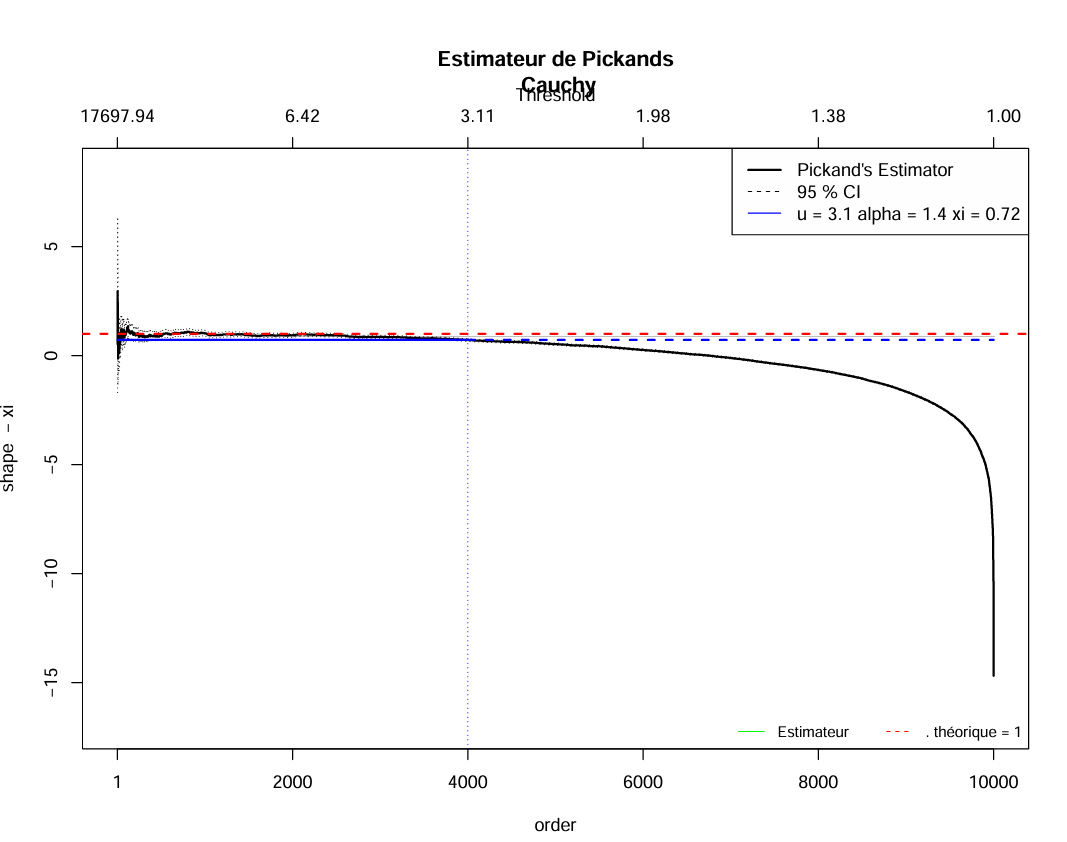
\includegraphics[width=0.8\textwidth]{./images/cauchy.png}
    \caption{Estimateur de Pickands pour la distribution de Cauchy.}
    \label{fig:pickands_cauchy}
\end{figure}

La figure \ref{fig:pickands_cauchy} présente l’estimateur de Pickands appliqué à un échantillon de loi de Cauchy. Cette loi est caractérisée par une queue extrêmement lourde et appartient au domaine d’attraction de Fréchet, avec un indice de queue théorique \(\gamma = 1\).

Le comportement de l’estimateur est ici particulièrement intéressant. Pour les faibles valeurs de \(k\), l’estimateur est très instable, ce qui est attendu compte tenu de la nature explosive des grandes valeurs dans une loi de Cauchy. À partir d’un certain seuil (environ \(k = 500\)), une phase de stabilisation est visible, avec une estimation qui reste relativement proche de la valeur attendue.

Cependant, on note qu’au-delà de \(k \approx 4000\), l’estimateur décroît significativement. Cela s’explique par le fait que l’inclusion d’observations moins extrêmes perturbe la qualité de l’estimation.
Ainsi, le cas de la Cauchy montre bien les limites pratiques de l’estimateur, malgré sa validité théorique.

\subsubsection{Synthèse}
Ces représentations graphiques montrent que l’estimateur de Pickands parvient globalement à capturer l’indice de queue \(\gamma\) pour différentes familles de distributions. Il converge correctement pour les cas classiques (Pareto, exponentielle), mais présente une instabilité accrue pour les queues bornées ou très lourdes. Ces résultats illustrent à la fois les points forts et les limites de l’estimateur, notamment sa sensibilité au choix de \(k\).

\subsection{Construction de l'estimateur de Pickands}
\textbf{Proposition :} (Caractérisations de \( D(H_{\gamma}) \))

Pour \( \gamma \in \mathbb{R} \), les affirmations suivantes sont équivalentes. \newline
\( (a) \quad F \in D(H_{\gamma}) \) \newline
\( (b) \) Pour une certaine fonction positive \( c(t) = a\left( \frac{1}{t} \right) \) :

\[
\lim_{t \to 0} \frac{U(tx) - U(t)}{c(t)} = 
\begin{cases} 
\frac{x^\gamma - 1}{\gamma} & \text{si } \gamma \neq 0, \\
\log(x) & \text{si } \gamma = 0, 
\end{cases}
\quad \text{pour } x > 0.
\]
La dernière affirmation est équivalente à :
\[
\lim_{s \to 0} \frac{U(sx) - U(s)}{U(sy) - U(s)} = 
\begin{cases} 
\frac{x^\gamma - 1}{y^\gamma - 1} & \text{si } \gamma \neq 0, \\
\frac{\log(x)}{\log(y)} & \text{si } \gamma = 0.
\end{cases}
\]
pour \(x,y > 0\) et \(y \neq 1\). \newline

\textbf{Lemme A:}
Soit \(X_1, \dots, X_n\) des variables aléatoires indépendantes et de fonction de répartition \(F\).
Soit \(U_1, \dots, U_n\) des variables aléatoires indépendantes de loi uniforme \(\left[0,1\right]\). Alors \(F^{-1}(U_{1,n}), \dots, F^{-1}(U_{n,n})\) a même loi que \((X_{1,n}, \dots, X_{n,n})\)\newline
\textbf{Preuve de la construction de l'estimateur de Pickands :}

On déduit de la proposition précédente que pour $\gamma \in \mathbb{R}$ et $\alpha$ on a avec le choix $t = 2s$, $x = 2$ et $y = \frac{1}{2}$,
\[
\lim_{t \to \infty} \frac{U(t) - U(t/2)}{U(t/2) - U(t/4)} = 2^{\gamma}.
\]

En fait, en utilisant la croissance de $U$ qui se déduit de la croissance de $F$, on obtient
\[
\lim_{t \to \infty} \frac{U(t) - U(t_{c_1}(t))}{U(t_{c_1}(t)) - U(t_{c_2}(t))} = 2^{\gamma}
\]
dès que $\lim_{t \to \infty} c_1(t) = \frac{1}{2}$ et $\lim_{t \to \infty} c_2(t) = \frac{1}{4}$. Il reste donc à trouver des estimateurs pour $U(t)$.

Soit $k(n), n \geq 1$ une suite d’entiers telle que $1 \leq k(n) \leq \frac{n}{4}$ et $\lim_{n \to \infty} \frac{k(n)}{n} = 0$ et $\lim_{n \to \infty} k(n) = \infty$.

Soit $(V_{1,n},\dots,V_{n,n})$ la statistique d’ordre d’un échantillon de variables aléatoires indépendantes de loi de Pareto. On note $F_V(x) = 1 - x^{-1}, x \geq 1$.

On déduit avec certains résultats de bases liés à $(V_{1,n},\dots,V_{n,n})$ que les suites
\[
\frac{k}{n} V_{n-k+1,n}, \quad \frac{2k}{n} V_{n-2k+1,n}, \quad \frac{4k}{n} V_{n-4k+1,n}
\]
pour \(n \geq 1\) convergent en probabilité vers 1.

On en déduit en particulier, les convergences en probabilité suivantes :
\[
V_{n-k+1,n}  \to \infty, \quad \frac{V_{n-2k+1,n}}{V_{n-k+1,n}} \to \frac{1}{2}, \quad \frac{V_{n-4k+1,n}}{V_{n-k+1,n}} \to \frac{1}{4}.
\]

Donc la convergence suivante a lieu en probabilité :
\[
\frac{U(V_{n-k+1,n}) - U(V_{n-2k+1,n})}{U(V_{n-2k+1,n}) - U(V_{n-4k+1,n})} \to 2^{\gamma}.
\]

Remarquons que si $x \geq 1$, alors $U(x) = F^{-1}(F_V(x))$. On a donc
\[
(U(V_{1,n}), \dots, U(V_{n,n})) = (F^{-1}(F_V(V_{1,n})), \dots, F^{-1}(F_V(V_{n,n}))).
\]

Or \(F_V\) est la fonction de répartition de la loi de Pareto. \newline
On déduit de la croissance de $F_V$ que $(F^{-1}(F_V(V_{1,n})),\dots, F^{-1}(F_V(V_{n,n})))$ a la même loi qu’une suite de $n$ variables aléatoires uniformes sur $[0,1]$ indépendantes. 

On déduit du lemme A que le vecteur aléatoire $(F^{-1}(F_V(V_{1,n})),\dots, F^{-1}(F_V(V_{n,n})))$ a la même loi que $(X_1,\dots,X_n)$. 

Donc la variable aléatoire \(\frac{U(V_{n-k+1,n}) - U(V_{n-2k+1,n})}{U(V_{n-k+1,n}) - U(V_{n-4k+1,n})}\) a la même loi que :

\[
\frac{X_{n-k+1,n} - X_{n-2k+1,n}}{X_{n-k+1,n} - X_{n-4k+1,n}}
\]

Ainsi cette quantité converge en loi vers $2^{\gamma}$ quand $n$ tend vers l’infini.

\subsection{Estimateur de Hill}
Cet estimateur a été introduit par Hill en 1975 dans le but d’estimer, de manière non paramétrique, le paramètre de queue des lois appartenant au domaine d’attraction de Fréchet. Il offre une estimation de l’indice de queue généralement plus efficace que celle fournie par l’estimateur de Pickands. La construction de cet estimateur repose sur l’utilisation des $k_n$ plus grandes statistiques d’ordre de l’échantillon.
\section*{La construction de l’estimateur de Hill}

Soient $\alpha_n$ et $\beta_n$ deux suites de nombres positifs, la construction de l’estimateur de Hill basée sur la relation suivante :

\begin{equation}
    q_{\beta_n} \simeq q_{\alpha_n} \left( \frac{\alpha_n}{\beta_n} \right)^{\gamma}.
    \tag{1.6}
\end{equation}

Passons au logarithme dans l’équation (1.6), ce qui donne :

\[
\log(q_{\beta_n}) - \log(q_{\alpha_n}) \simeq \gamma \log\left( \frac{\alpha_n}{\beta_n} \right).
\]

On choisit $\alpha_n = k_n/n$ et on considère plusieurs valeurs pour $\beta_n$, $\beta_n = i/n$ avec $i = 1, \ldots, k_n - 1$ tout en ayant $\beta_n < \alpha_n$. On obtient alors :

\[
\log(q_{i/n}) - \log(q_{k_n/n}) \simeq \gamma \log(k_n/i).
\]

Ainsi, en estimant les quantiles par leurs équivalents empiriques, on obtient :

\[
\log(X_{n - i + 1, n}) - \log(X_{n - k_n + 1, n}) \simeq \gamma \log(k_n / i).
\]

En sommant de part et d’autre sur $i = 1, \ldots, k_n - 1$, on obtient :

\[
\gamma = \frac{\displaystyle \sum_{i=1}^{k_n - 1} \log(X_{n - i + 1, n}) - \log(X_{n - k_n + 1, n})}{\displaystyle \sum_{i=1}^{k_n - 1} \log(k_n / i)}.
\]

Le dénominateur se réécrit $\log(k_n^{k_n - 1}/(k_n - 1)!)$. En utilisant la formule de Stirling, il est équivalent à $k_n$ au voisinage de l’infini. On obtient alors l’estimateur de Hill.

Soit $(k_n)_{n \geq 1}$ une suite d'entiers avec $1 \leq k_n \leq n$, l’estimateur de Hill est défini par :

\[
\hat{\gamma}^{H}_{k_n} = \frac{1}{k_n - 1} \sum_{i=1}^{k_n - 1} \log(X_{n - i + 1, n}) - \log(X_{n - k_n + 1, n}).
\]

L’estimateur de Hill satisfait la propriété de consistance faible. Plus précisément, si $(k_n)_{n \geq 1}$ est une suite intermédiaire, alors l’estimateur $\hat{\gamma}^{H}_{k_n}$ converge en probabilité vers le paramètre de queue $\gamma$, c’est-à-dire :
\[
\hat{\gamma}^{H}_{k_n} \xrightarrow{\mathbb{P}} \gamma.
\]


\subsection{Le choix du nombre de statistiques d’ordre}

Dans la pratique, déterminer une valeur appropriée pour le paramètre $k_n$, c’est-à-dire le nombre de plus grandes observations à retenir, constitue une étape délicate. Il faut en effet trouver un compromis entre la variance et le biais : utiliser suffisamment de données pour obtenir une estimation fiable, tout en s’assurant que ces données proviennent bien de la queue de la distribution. Diverses approches ont été développées dans la littérature pour guider ce choix.

\subsection{Comportement empirique de l’estimateur de Hill}

Nous présentons ci-dessous des représentations graphiques de l’estimateur de Hill appliqué à des échantillons de taille $n = 40000$ générés à partir de quatre lois différentes : Pareto, exponentielle, uniforme et Cauchy. Pour chacune d’elles, nous comparons les valeurs estimées de l’indice de queue $\gamma$ à leur valeur théorique.

\paragraph{Loi de Pareto :}
\begin{figure}[H]
    \centering
    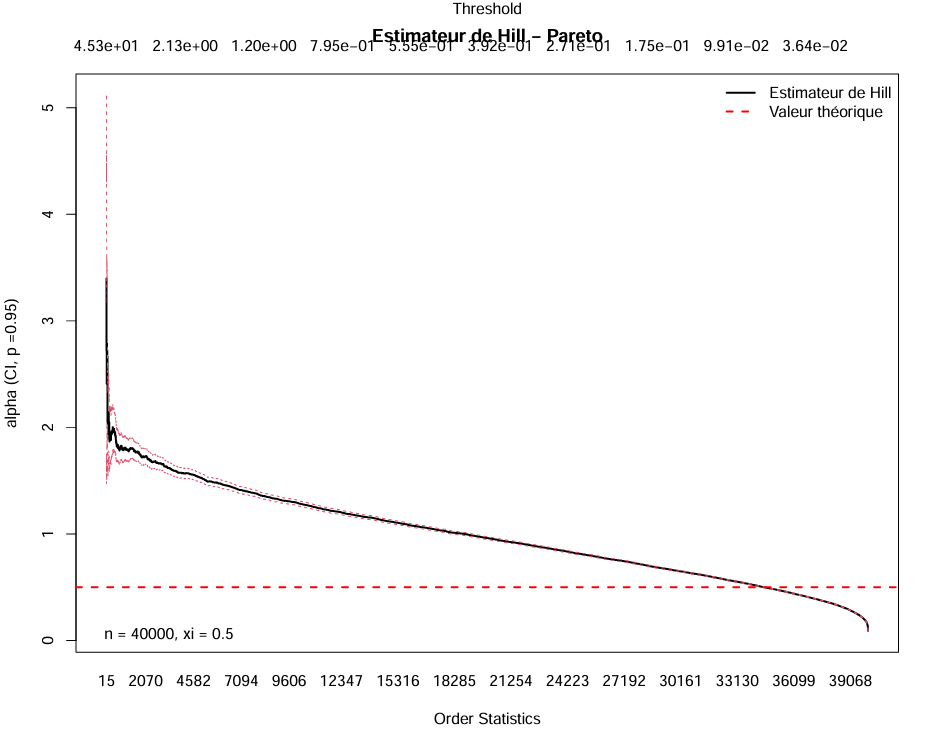
\includegraphics[width=0.6\textwidth]{./images/hill_pareto.png}
    \caption{Estimateur de Hill — Loi de Pareto ($\gamma = 0{,}5$)}
\end{figure}

Dans ce cas, la loi suit un comportement de queue lourde avec un indice théorique $\gamma = 0.5$, ce qui correspond parfaitement aux hypothèses de l’estimateur de Hill. Comme le montre la Figure, l’estimation converge de manière satisfaisante vers la valeur théorique pour un intervalle raisonnable de seuils $k$. On observe une certaine instabilité pour les petites valeurs de $k$, mais une fois la courbe stabilisée, elle oscille autour de la vraie valeur. Ce comportement valide l'efficacité de l’estimateur dans ce cadre.
\paragraph{Loi exponentielle :}
\begin{figure}[H]
    \centering
    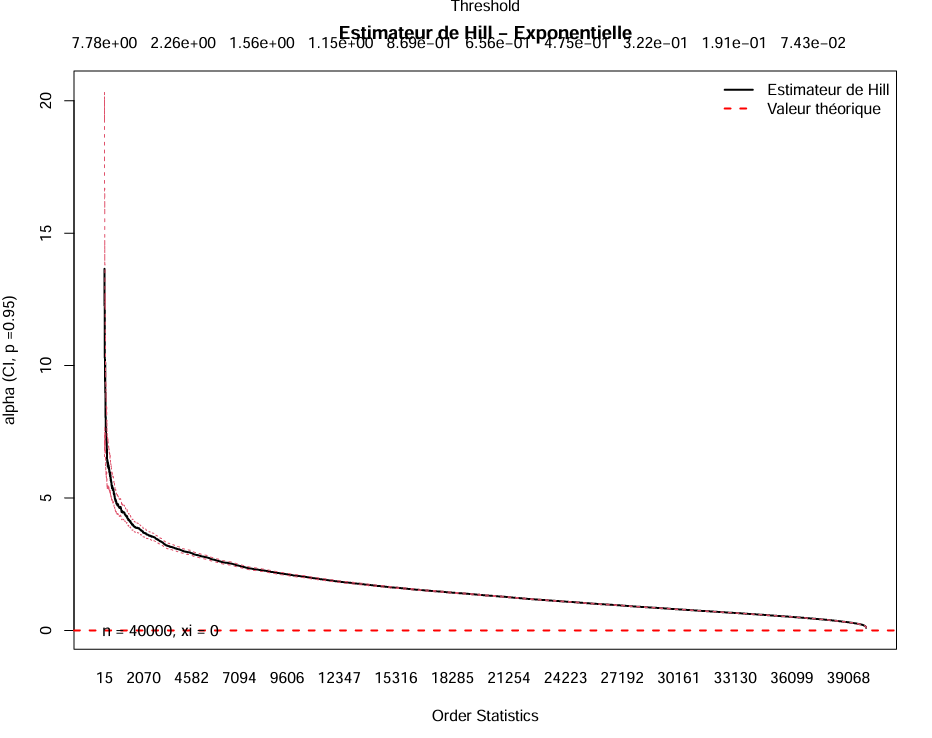
\includegraphics[width=0.6\textwidth]{./images/hill_expo.png}
    \caption{Estimateur de Hill — Loi exponentielle ($\gamma = 0$)}
\end{figure}

La loi exponentielle appartient au domaine de Gumbel, avec un indice de queue $\gamma = 0$. L’estimateur de Hill n’est pas adapté à ce domaine. Le graphique le confirme clairement : la courbe estimée commence avec des valeurs très élevées, puis décroît lentement sans jamais converger vers la valeur théorique nulle. L’absence de convergence met en évidence l’inadéquation de l’estimateur dans ce contexte.
\paragraph{Loi uniforme :}
\begin{figure}[H]
    \centering
    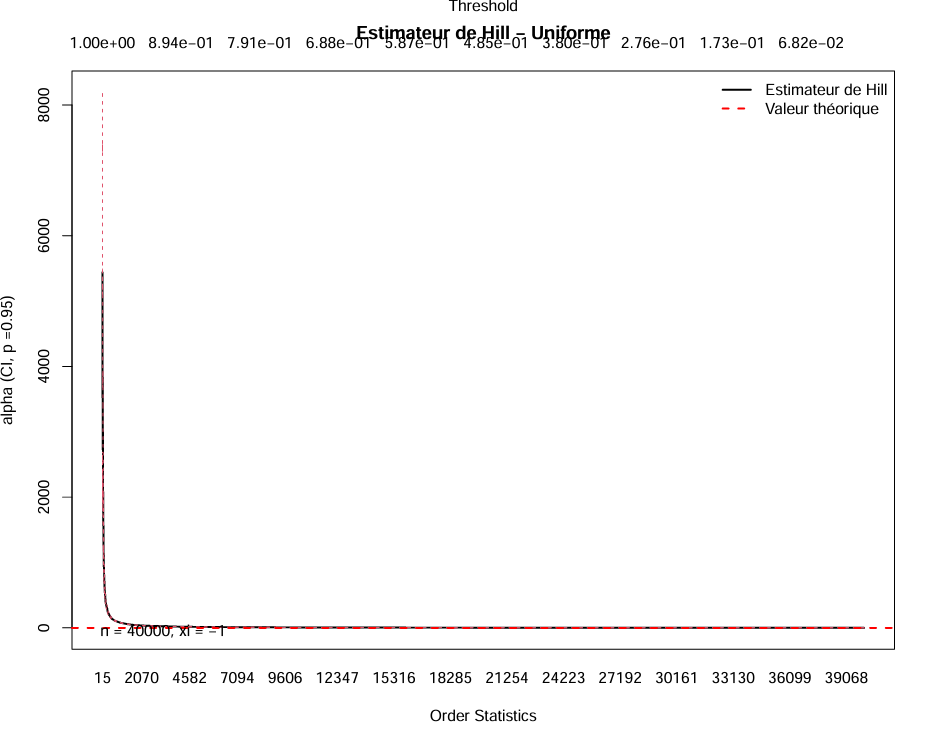
\includegraphics[width=0.6\textwidth]{./images/hill_uniforme.png}
    \caption{Estimateur de Hill — Loi uniforme ($\gamma = -1$)}
\end{figure}

Cette loi présente une queue bornée, avec un indice $\gamma = -1$, ce qui sort du domaine d’application de Hill. L’estimateur suppose en effet que $\gamma > 0$. Le graphique montre une estimation extrêmement instable, avec des valeurs incohérentes, souvent très grandes ou très faibles, indiquant que le modèle n’est pas du tout approprié à ce type de données. 
\paragraph{Loi de Cauchy :}
\begin{figure}[H]
    \centering
    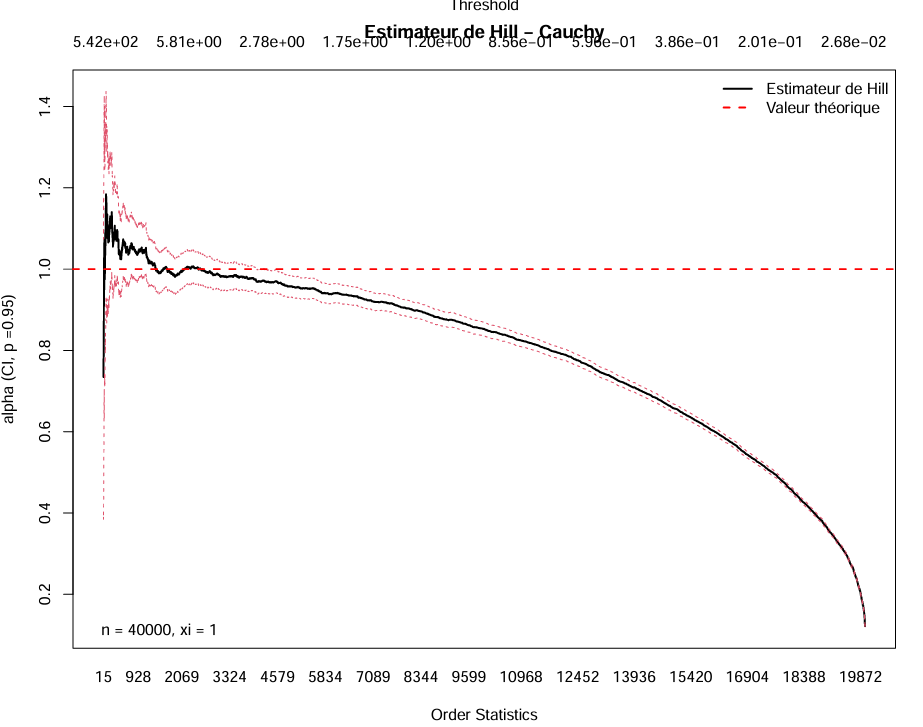
\includegraphics[width=0.6\textwidth]{./images/hill_cauchy.png}
    \caption{Estimateur de Hill — Loi de Cauchy ($\gamma = 1$)}
\end{figure}

La distribution de Cauchy, avec un indice $\gamma = 1$, est dans le domaine de Fréchet, donc en principe bien adaptée à l’estimateur de Hill. Le graphique montre une bonne estimation dans les faibles valeurs de $k$, la courbe noire se stabilisant autour de la valeur théorique. Cependant, dès que $k$ devient trop grand, l’estimation chute fortement, trahissant un biais introduit par l'inclusion d’observations moins extrêmes. Ce phénomène illustre la sensibilité de l’estimateur au choix du seuil $k$.
\medskip

En résumé, ces observations soulignent la pertinence de l’estimateur de Hill pour les lois à queue lourde (Pareto, Cauchy), et son inadéquation manifeste pour les lois à queue légère ou bornée (exponentielle, uniforme). Le choix judicieux du paramètre $k$ demeure également crucial pour obtenir une estimation fiable.

\subsection{Estimateur de DEDH}
Le troisième estimateur de l'indice de queue est celui proposé par Dekkers, Einmahl et De Haan. Il s'agit d'une généralisation de l'estimateur de Hill, applicable à tous les domaines d'attraction. Il est défini par :

\[
\hat{\gamma}_n^{(DEdH)}(k_n) = \mathcal{M}^{(1)}_{k_n} + 1 - \frac{1}{2} \left( 1 - \frac{(\mathcal{M}^{(1)}_{k_n})^2}{\mathcal{M}^{(2)}_{k_n}} \right)^{-1}
\]

où 
\[
\mathcal{M}^{(r)}_{k_n} = \frac{1}{k_n} \sum_{i=1}^{k_n} (\ln(X_{(n-i+1)}) - \ln(X_{(n-k_n)}))^r.
\]
La valeur de \(\mathcal{M}^{(1)}_{k_n}\) correspond à l'estimateur de Hill.

L'estimateur de DEDH possède la propriété de convergence en loi :

\[
\sqrt{k_n}(\frac{\hat{\gamma}_n^{(DEdH)}(k_n) - \gamma}{\sigma_M}) \xrightarrow{\mathcal{L}} \mathcal{N}(0,1) \quad \text{quand } n \to \infty.
\]

où :

\[
\sigma_M^2 = 
\begin{cases} 
1 + \gamma^2, & \text{si } \gamma \geq 0, \\ 
(1 - \gamma^2)(1 - 2\gamma)
\left( 4 - \frac{8 (1 - 2\gamma)}{1 - 3\gamma} - \frac{(5 - 11\gamma)(1 - 2\gamma)}{(1 - 3\gamma)(1 - 4\gamma)} \right), 
& \text{si } \gamma < 0.
\end{cases}
\]

En pratique, il est difficile de comparer ces estimateurs de manière tranchée. Toutefois, l'estimateur de Hill se distingue par une variance asymptotique plus faible, ce qui justifie son choix dans la suite. Étant donné que cet estimateur n'est valide uniquement pour les distributions appartenant au domaine d'attraction de Fréchet, c'est-à-dire dans le cas où \(\gamma > 0\), il est essentiel de vérifier cette hypothèse. 

\section{Sélection des estimateurs de l'indice de valeurs extrêmes}

Le choix de l’estimateur dépend du type de distribution sous-jacente. L’estimateur de Hill est spécifiquement adapté aux distributions de Fréchet (\(\gamma > 0\)), caractérisées par des queues lourdes. Il est donc plus efficace dans ce cas et sera préféré à l’estimateur de Pickands.  

Cependant, pour les distributions de Weibull (\(\gamma < 0\)) et Gumbel (\(\gamma = 0\)), l’estimateur de Hill n’est pas applicable. Dans ces cas, on utilise l’estimateur de Pickands, qui est valide quel que soit le signe de \( \gamma \).  

L'estimateur de Pickands est basé sur les distances entre deux statistiques d'ordre, sans tenir compte du maximum de l’échantillon, ce qui entraîne une perte d'information sur la queue de distribution. Par conséquent, il présente une plus grande volatilité que l'estimateur de Hill, qui repose sur la moyenne des logarithmes des observations.

\newpage
\section{Application sur des données réelles}

Afin d'illustrer les méthodes d'estimation de l'indice de valeurs extrêmes, nous allons appliquer ces techniques sur des données réelles.
Nous allons utiliser les données du package $ismev$ de R. Plus précisément wooster et rain. Wooster contient les données de température minimale (en Fahrenheit) annuelle à Wooster de 1983 à 1988.
Tandis que Rain contient les données de pluie journalière dans en Angleterre de 1914 à 1962.
\\
Nous allons utiliser deux méthodes d'estimation sur les paramètres $a_n$, $b_n$ et $\gamma$ afin de d'estimer la valeur extrême.

\subsection{Première méthode (Méthode des maxima en bloc) avec Wooster}
\subsubsection{Principe}

La première étape consiste à découper nos données en blocs de taille $k$ et de calculer le maximum sur chaque bloc. Le paramètre
$k$ est choisit en fonction de l'interprétation des données. (par exemple, si on a des données journalières, on peut choisir $k=365$ pour avoir des maximums annuels).
Ensuite, pour chaque bloc on calcule le maximum. Cela nous donne une suite de maximum.
Une fois les maximums obtenus, on estime $a_n$,$b_n$ et $\gamma$ en utilisant la méthode du maximum de vraisemblance.

\subsubsection{Application sur les données de Wooster}
L'objectif sur ces données est de savoir s'il existe (et dans le cas échéant de le calculer) un seuil tel que les températures ne puissent pas dépasser.
Chercher cette valeur seuil serait utile en agriculture par exemple pour savoir si les températures ne sont pas trop élevées pour les cultures.

\begin{center}
	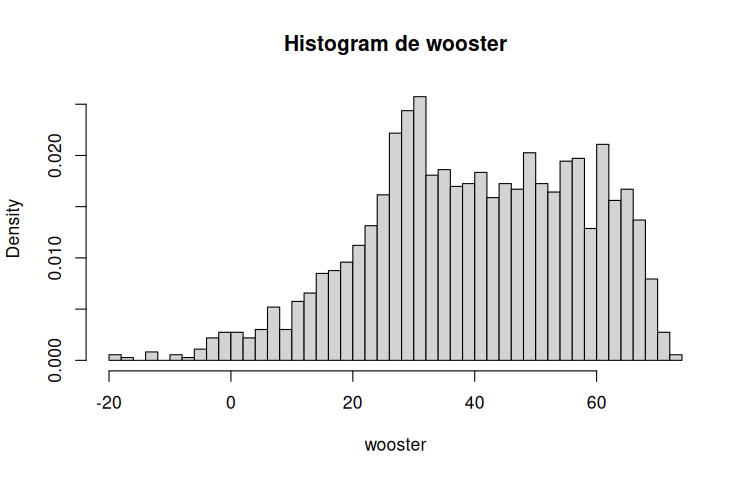
\includegraphics[scale=0.8]{./images/woosterhisto.png} 
\end{center}

Nous avons découper ici nos données en blocs de taille $60$ et de calculer le maximum sur chaque bloc.
L'estimation numériques par l'algorithme de Nelder-Mead des paramètres $a_n$,$b_n$  (qu'on note pour la suite $\sigma$ et $\mu$) et $\gamma$ nous donne :
\[
\sigma = 36.02, \quad \mu= 18.82, \quad \gamma = -0.5
\]

Nous obtenons une valeur de $\gamma$ négative, ce qui signifie que la distribution des températures max à Wooster est de type Weibull.
Nous pouvons donc conclure que les températures à Wooster sont pas limitées par un seuil.
Ce seuil étant donnée dans la partie 1, il vaut : $x_{max} = \mu - \frac{\sigma}{\gamma} = 74.93 $
\\
\\
Il est alors raisonnables de penser que les températures à Wooster ne dépassent pas $74.93$.

v
\subsection{Méthode de dépassement de seuil avec \textbf{Rain}}

\subsubsection{Principe}

La deuxième méthode consiste à fixer un seuil $u$ et de considérer les données qui dépassent ce seuil. C'est à dire $X_i$ tel que $X_i > u$.
Ensuite, on stocke les excès $X_i - u$. Cela nous donne un jeu de données positifs.
La clé de cette méthode est que pour un seuil $u$ bien choisi, les excès suivent une loi de Pareto de paramètres $\sigma$ (échelle) et $\gamma$ (le gamma qu'on estime dans toute la théorie).
C'est alors qu'on ajuste les paramètres $\sigma$ et $\gamma$ par maximum de vraisemblance.

\subsubsection{Application sur les données de Rain}

L'objectif sur ces données est de savoir s'il existe (et le cas échéant de le calculer) un seuil tel que les pluies ne puissent pas dépasser.
Chercher cette valeur seuil serait utile en agriculture par exemple pour savoir si les pluies ne sont pas trop élevées pour les cultures.

\begin{center}
	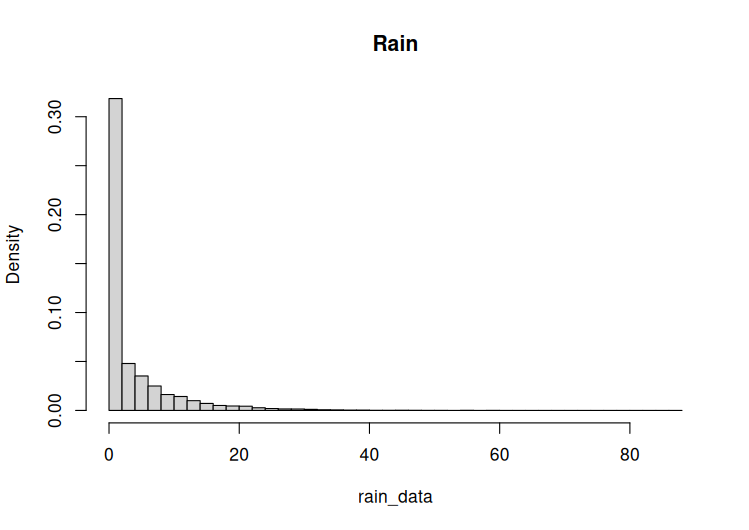
\includegraphics[scale=0.8]{./images/rainhisto.png} 
\end{center}

On remarque dans un premier temps que les données sont concentrées autour de 0 mais qu'elles sont capables de prendre des valeurs très élevées.
Il est alors raisonnable de penser qu'après estimation, on va obtenir une valeur de gamma positive ou nulle. En effet, il n'apparait pas de cassure dans la distribution des données.
De plus, la queue de distribution est longue mais ne parait pas lourde. Ce qui suggèrerait une valeur de gamma proche de 0.
\\
\\
Après estimation numérique, on obtient : $\sigma = 7.94$ et $\gamma = 0.034$ avec pour $\gamma$ un intervalle de confiance : $[-0.022 ; 0.102]$.
\\
\\ 
Une valeur de gamma aussi proche de 0 doit nous conduire à une étude plus approfondie.
Plusieurs méthodes s'offrent à nous pour améliorer l'estimation de gamma. 
\\
ON Peut considère la première méthode afin de comparer les résultats.
\\
On peut faire varier le seuil $u$ et juger de l'impact sur l'estimation de gamma.
\\
Ou alors de façon plus arbitraire, on peut considérer la valeur de gamma en fonction du type de donnée qu'on étudie et de la cohérence que cela apporte.
\\
\\
\\
Pour notre exemple, on considère que $\gamma > 0$

\begin{center}
	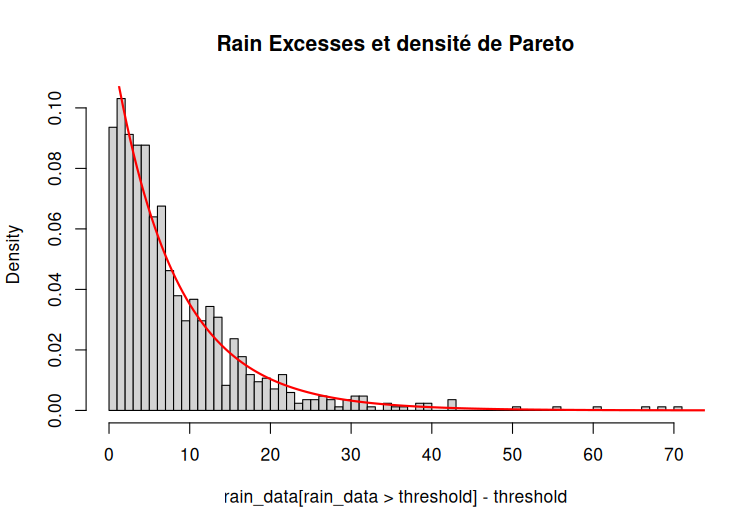
\includegraphics[scale=0.8]{./images/rainhistodensite.png} 
\end{center}

La distribution de Pareto (courbe rouge) avec les paramètres estimés semblent bien coller avec les données. Cela signifie qu’on s’attend à des excès au-delà du seuil de plus en plus rares, sans pour autant exclure la survenue de précipitations sensiblement élevées.
\\
\\
L'avantage de cette méthode est qu'elle est plus efficace car elle utilise plus de données. Cependant, elle est plus difficile à mettre en place car il faut choisir un seuil $u$ qui est crucial pour l'estimation de gamma.


\subsubsection{Méthode de Nelder-Mead}

\noindent Le package "evd", que nous avons utilisé pour réaliser les méthodes de dépassement de seuil et des maxima en bloc, utilise l'algorithme de Nelder-Mead pour calculer les paramètres de la fonction limite et ainsi savoir dans quel cas où se trouve : Fréchet, Gumbel ou Weibull. \\

\noindent Nelder-Mead est un algorithme d'optimisation non linéaire, il consiste en la chose suivante dans le cadre des valeurs extrêmes : 
\begin{itemize}
	\item \textbf{Etape 1} : on commence par choisir 3 premiers points $x_1, x_2, x_3$ par une rapide estimation des paramètres $\sigma$, $\mu$ et $\gamma$ de nos données. Ce seront nos points de départs de l'algorithme et ils définissent notre premier simplexe (triangle ici) dans $R^2$.
	\item \textbf{Etape 2} : on calcule ensuite la valeur de la fonction en ces 3 points : f est la fonction GEV généralisée (à définir plus précisément) et on les trie par valeurs décroissantes.
	\item \textbf{Etape 3} : on cherche le centre de gravité $x_0$ de nos premiers points : $x_0 = \frac{x_1 + x_2 + x_3}{3}$.
	\item \textbf{Etape 4} : on fait ensuite une réflexion en calculant $x_r = x_0 + \alpha (x_0 - x_3)$ où $\alpha > 0$ est appelé le coefficient de réflexion
	\item \textbf{Etape 5} : si $f(x_1) \le  f(x_r) \le  f(x_3)$ : on remplace $x_3$ par $x_r$ et on retourne à l'étape 2.
	\item \textbf{Etape 6} : si $f(x_r) \le  f(x_1)$ : on procède à une expansion du simplexe, on calcule $x_3 = x_0 + \gamma(x_r - x_0)$ où $\gamma > 1$. Si $f(x_e) \le  f(x_r) $, on remplace $x_3$ par $x_e$ sinon on remplace $x_3$ par $x_r$ et on retourne à l'étape 2
	\item \textbf{Etape 7} : si $f(x_r) \geq f(x_3)$ : on procède à une contraction du simplexe, on cherche $x_c = x_0 + \rho(x_3 - x_0)$ où $0 < \rho < 0.5 $ . Si $f(x_c) \le  f(x_3)$, on remplace $x_3$ par $x_c$ et on retourne à l'étape 2, sinon on continue jusqu'à l'étape 8.
	\item \textbf{Etape 8} : on effectue une homothétie de rapport $\omega$ et de centre $x_1$ : on remplace ainsi $x_i$ par $x_1 + \omega(x_i - x_1)$ où $0 < \omega < 1$et on retourne à l'étape 2
\end{itemize}

\noindent On répète cela jusqu'à atteinte du critère d'arrêt, en général : $ \sqrt{\sum_{i=1}^{n+1}  \frac{(f_i - \bar{f})^2}{n}} < \epsilon $ où $\bar{f} =\frac{1}{n+1} \sum_{i=1}^{n+1} f_i $ et $ \epsilon $ est un réel proche de 0. \\

\newpage
\section{Annexe}

\subsection{Codes R}

\noindent Voici un exemple de code R utilisé dans la première section :

\begin{lstlisting}
	# Paramètres
	n <- 1000        # Taille de l'échantillon pour la simulation des lois uniformes
	N <- 10000       # Nombre de simulations pour le maximum
	
	# Simulation des maxima de lois uniformes(0,1)
	set.seed(123)    # fixation de l'aléa
	M_n <- replicate(N, max(runif(n))) # M_n = max / X_n = runif
	
	# Normalisation pour observer la convergence
	Y_n <- n * (1 - M_n)
	
	# Histogramme des valeurs transformées
	hist(Y_n, breaks = 50, probability = TRUE, 
	col = "lightblue", border = "white", ylab = "Densité",
	xlab = expression(Y_n), main = "Max de 1000 lois uniformes")
	
	# Densité théorique de la loi exponentielle (paramètre = 1)
	curve(dexp(x, rate = 1), col = "red", lwd = 2, add = TRUE)
	
	# Légende
	legend("topright", legend = c("Simulation", "Densité théorique : exp(1)"),
	fill = c("lightblue", NA), border = c("white", NA), 
	lty = c(NA, 1), col = c(NA, "red"), lwd = c(NA, 2))
\end{lstlisting}

\begin{lstlisting}
	#################### CODE POUR WOOSTER ####################
	library(ismev)
	library(evd)
	data("wooster")
	
	gev_fit <- fgev(wooster)
	
	mu <- as.numeric(gev_fit$param[1])
	sigma <- as.numeric(gev_fit$param[2])
	gamma <- as.numeric(gev_fit$param[3])
	
	# estimation de gamma avec pickands (juste pour comparer)
	
	x <- sort(wooster)
	n <- length(x)
	k <- floor(0.1 * length(wooster))
	X1 <- x[n - k + 1]
	X2 <- x[n - 2*k + 1]
	X3 <- x[n - 4*k + 1]
	pickands_est <- (1 / log(2)) * log((X1 - X2) / (X2 - X3))
	print(pickands_est)
	
	
	# gamma est < 0 donc on calcule la borne max
	x_max <- mu - sigma / gamma
	
	# Définir la densité de la loi (pour gamma < 0)
	dgev <- function(x, mu, sigma, gamma) {
	  t <- 1 + gamma * ((x - mu) / sigma)
	  dens <- ifelse(t > 0, 
					 (1/sigma) * t^(-1/gamma - 1) * exp(-t^(-1/gamma)), 
					 0)
	  return(dens)
	}
	
	xseq <- seq(min(wooster), max(wooster), length.out = 200)
	
	# PLOT   
	
	hist(wooster,main = "Histogram de wooster" ,breaks = 60, probability = TRUE, col = "lightgray")
	
	lines(xseq, dgev(xseq, mu, sigma, gamma), col = "blue", lwd = 2)
	
	
	abline(v = x_max, col = "red", lwd = 2, lty = 2)
	legend("topright", legend = paste("x_max =", round(x_max, 2)), col = "red", lwd = 2, lty = 2)
	
	# plot plus détaillé
	plot(gev_fit)



	
\end{lstlisting}

\begin{lstlisting}
	#################### CODE POUR RAIN ####################
	library(ismev)
	library(evd)
	data(rain)
	rain_data <- rain

	# seuil	
	threshold <- quantile(rain_data, probs = 0.95)
	gpd_result <- gpd.fit(rain_data, threshold)

	# on stocke la parametre d'échelle et de forme
	sigma <- gpd_result$mle[1]
	gamma <- gpd_result$mle[2]
	SE <- gpd_result$se[2]
	IC <- c(gamma - 1.96 * SE, gamma + 1.96 * SE)    # contient 0 (oups)


	# On code la fonction de pareto généralisée parametre echel sigma et de forme gamma
	pareto <- function(x, gamma, sigma) {
	  if (gamma == 0) {
		return(1/sigma * exp(-x/sigma))
	  } else {
		return(1/sigma * (1 + gamma * x/sigma)^(-1/gamma - 1))
	  }
	}

	# on trace l'histogramme des données
	hist(rain_data, breaks = 50, freq = FALSE, main = "Rain")

	# on trace l'histogramme des données en excés par rapport au seuil et la loi de pareto
	hist(rain_data[rain_data > threshold] - threshold, breaks = 50, freq = FALSE, main = "Rain Excesses et densité de Pareto")

	# on trace la loi de gpd avec les paramètres estimés
	xseq <- seq(min(rain), max(rain), length.out = 200)
	lines(xseq, pareto(xseq, gamma, sigma),col='red', lwd=2)



	# pour le qq-plot et residus
	gpd.diag(gpd_result)

\end{lstlisting}
\end{document}